
\chapter{Teoría Fractal}
\hrule \bigskip \vspace*{1cm}



\section{Introducción}

Un Fractal es definido como un objeto que presenta aproximadamente las mismas características
independientemente de la escala donde es analizada, es un objeto que se parece a si mismo, por otro lado, las partes del fractal son similares, exactas o estadísticas, a un completo fractal, los detalles en una escala pequeña son similares a las características de una gran escala.
\\\\
Por ejemplo, el triangulo Sierpinkski es un fractal geométrico, que ha sido construido en un proceso iterativo, teóricamente infinito, en un triangulo equilátera ABC, donde primero se ha removido el triangulo central A, B, C,  De cada uno de los tres triángulos restantes cuyos lados
Longitud igual a la mitad del lado de ABC, retiramos de nuevo el triángulo central. La figura \ref{fig:ima1} muestra los pasos iniciales del proceso de construcción de un triángulo de Sierpinski.
\\\\
El triángulo restante tiene "agujeros" independientemente de la escala y cada triángulo dentro de la primera
Es una "miniatura" de todo el triángulo.

\begin{figure}[h]
\centering
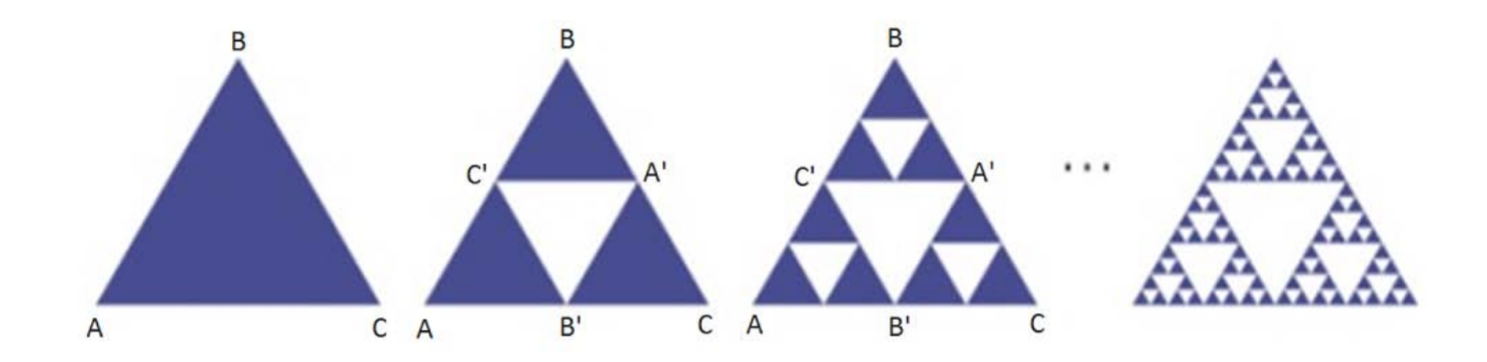
\includegraphics[scale=0.75]{chapter4/ima1.png}
\caption{Pasos del proceso de construccion del tiangulo de Sierpinsky}
\label{fig:ima1}
\end{figure}

Hay muchas otras estructuras matemáticas definidas como fractal, como el Koch
, El conjunto de Cantor y el conjunto de Mandelbrot que se presentan en la figura \ref{fig:ima2}.
\\\\
Son también ejemplos de fractales en la naturaleza, por ejemplo: nubes, montañas, hortalizas, árboles,
La costa de continentes, islas y otros

\begin{figure}[h]
\centering
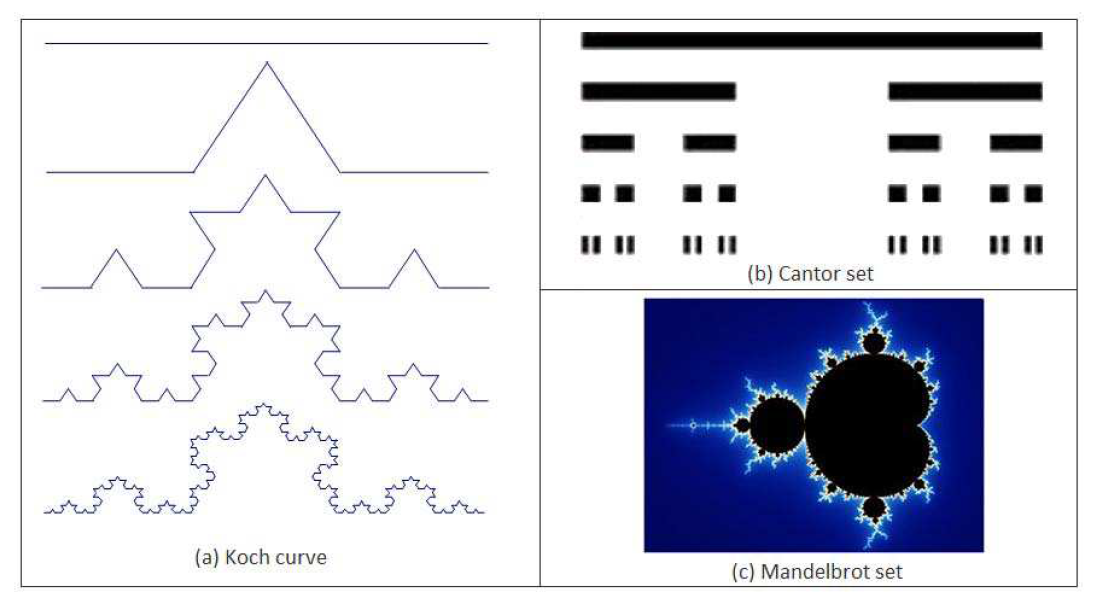
\includegraphics[scale=1.2]{chapter4/ima2.png}
\caption{Algunos ejemplos de fractales (a y b) fractales geométricos y (c) fractales algebraicos}
\label{fig:ima2}
\end{figure}


Los conceptos de fractal se han aplicado a varias tareas en el análisis de datos y la minería de datos.
\\\\
Una de ellas es la estimación de la dimensión intrínseca (D) del conjunto de datos, que es
Relacionado con el concepto de dimensión de inclusión (E) (Faloutsos & Kamel, 1994).
\\\\
\textbf{Definición 3.1 Incorporación de la dimensión E:} Dado un conjunto finito de datos A, la incorporación
Dimensión E ∈ N es el número de atributos que definen A, es decir, E es la dimensión de
El espacio en el que se incrusta el conjunto de datos.
\\\\
\textbf{Definición 3.2 Dimensión intrínseca D:} Dado un conjunto de datos finitos A, su dimensión intrínseca
D ∈ R +, es la dimensionalidad del objeto representado por los datos, independientemente de la
Dimensión del espacio en el que está incrustado.
\\\\
La dimensión intrínseca (D) es una medida de la cantidad de información que el conjunto de datos
Representa Por ejemplo, la dimensión intrínseca de un conjunto de puntos distribuidos
\\\\
La línea es igual a uno; Si el conjunto está incrustado en un espacio dimensional superior, el intrínseco
Dimensionalidad continúa igual a uno como se ilustra en la figura \ref{fig:ima3}.


\begin{figure}[h]
\centering
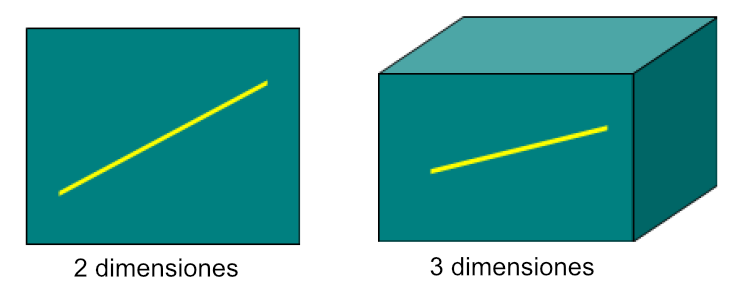
\includegraphics[scale=1.2]{chapter4/ima3.png}
\caption{Una lina enbebida in dos y tres dimensiones}
\label{fig:ima3}
\end{figure}


Faloutsos & Kamel (1994) propuso el uso de la dimensión intrínseca como una herramienta para
Medir el comportamiento no uniforme de conjuntos de datos reales. Además, los autores presentaron
Estudios empíricos para demostrar que los datos reales suelen tener un comportamiento
Es la característica fundamental de los objetos fractales. Por lo tanto, la dimensión intrínseca D
De un conjunto de datos real puede calcularse calculando su dimensión fractal.
\\\\
La dimensión intrínseca basada en la dimensión fractal ha sido empleada como una Herramienta para el análisis de agrupamiento (Barbar'a & Chen, 2003), minería de reglas de asociación temporal
(Barbar'a et al., 2004), selección de atributos (Traina Jr. et al., 2000, 2010), series cronológicas
(Chakrabarti y Faloutsos, 2002) y la minería de datos espaciales (Traina et al., 2001).
\\\\
En este capítulo presentamos los principales conceptos relacionados con la teoría
Utilizado en algunos de los métodos propuestos en esta tesis.
\\\\
La sección 2 muestra diferentes maneras de
Calcular la dimensión fractal. El cálculo de correlación indicado por la correlación
La Dimensión Fractal se detalla en la Sección 3 La teoría fractal empleada para monitorear los datos En la sección 3

\section{Dimensión fractal}

Los fractales suelen tener características inusuales que pueden considerarse paradojas. Por ejemplo,
El triángulo de Sierpinski tiene un perímetro infinito (proporcional a $lim_{i\rightarrow\infty} (1+1/2)^i  $ )
Y nulo (proporcional a $lim_{i\rightarrow\infty} (3/4)^i $) ya que a cada iteración de su proceso de construcción,
Que es teóricamente infinito, su perímetro aumenta y su área disminuye.
\\\\
Debido
A estas propiedades, este fractal no puede ser considerado un euclidiano unidimensional
Objeto (ya que su perímetro no es finito) ni un objeto bidimensional euclidiano (puesto que su
Área es nula). Así, es posible considerar una dimensionalidad de fraccionamiento llamada fractal
(Mandelbrot, 1983). Intuitivamente, la dimensión fractal del triángulo de Sierpinski es
Un valor entre 1 y 2. Matemáticamente, el valor preciso es 1,58.

\\\\
Hay varias definiciones para la dimensión fractal, que se presentan brevemente en este
sección. La medida básica de la dimensión fractal se dedica a los fractales denominados
Exactamente auto-similar. Este tipo de fractal se compone de $M$ réplicas que son cada uno
Una versión reducida 1: s del fractal original.
\\\\
\textbf{Definición 3.3 Dimensión fractal D:} Sea $M$ el número de réplicas y s la escala
Factor por el que se reduce cada réplica, la dimensión fractal D de una imagen exactamente igual Fractal definido en un espacio E-dimensional es:

\begin{equation}
D \equiv \frac{logM}{logs}
\label{eq:ec1}
\end{equation}

El triángulo de Sierpinski, por ejemplo, es un fractal exactamente auto-similar, porque su regla
De construcción genera tres réplicas en escala 1: 2 para cada iteración. Por lo tanto, la
Dimensión fractal de Sierpinski es$ D = \frac{log3}{log2} \approx 1.58$ Similarmente, en la Figura \ref{fig:ima2}
Cantor conjunto y la curva de Koch son exactamente fractales auto-similares con la dimensión fractal$ D = \frac{log2}{log3} \approx 0.63$ y $ D = \frac{log4}{log3} \approx 1.26$ respectivamente.

\\\\
Esta definición de la dimensión fractal D es adecuada para matemática exactamente auto-similar
Fractales con reglas de construcción recursivas bien definidas. Sin embargo, para conjuntos de datos llamados estadísticamente
Fractales auto-similares, que no tienen reglas de construcción bien definidas, es
Más apropiado para calcular la dimensión fractal mediante el método de recuento de cuadros
(Schroeder, 1991), que define la Dimensión Fractal de Correlación D2 tal como se presenta en
Ecuación \ref{eq:ec2}
\\\\

\textbf{Definición 3.4 Correlación Dimensión Fractal D2:} Dado un conjunto de datos auto-similar en
El rango de escalas $[r1, r2]$, su dimensión fractal de correlación $D_2 \rightarrow \left[ \mathbb{R}^{+} \right]$ se mide como

\begin{equation}
D_2 \equiv  \frac{\partial log (\sum_i C_{r,1}^2)}{\partial (r)} \qquad \:r \epsilon [r1,r2 ]
\label{eq:ec2}
\end{equation}

Donde r es el lado de las células en una (hiper) cuadrícula cúbica que divide el espacio de direcciones de la
Conjunto de datos, y $C_r,i$, i es el recuento de puntos en la i-ésima celda.

\\\\
De forma práctica, el valor derivado que define la dimensión fractal $D_2$ puede
Se obtiene mediante la construcción de la gráfica de recuento de bloques, que representa los valores de
$\sum_i C_{r,1}^2$  y $log (r)$ en un gráfico. Para los conjuntos de datos fractal, la curva resultante es lineal en
Un intervalo $(r1, r2)$ y la dimensión fractal D2 se estima por la pendiente de la línea que
Mejor se ajusta al intervalo analizado.
\\\\
La figura \ref{fig:ima4} muestra un conjunto de 6561 puntos en el Sierpinski
Triángulo y la parcela en la escala log-log de la suma de la ocupación cuadrada $\sum_i C_{r,1}^2$ contra el
Tamaño de la celda de la rejilla (radio) $r$.

\begin{figure}[h]
\centering
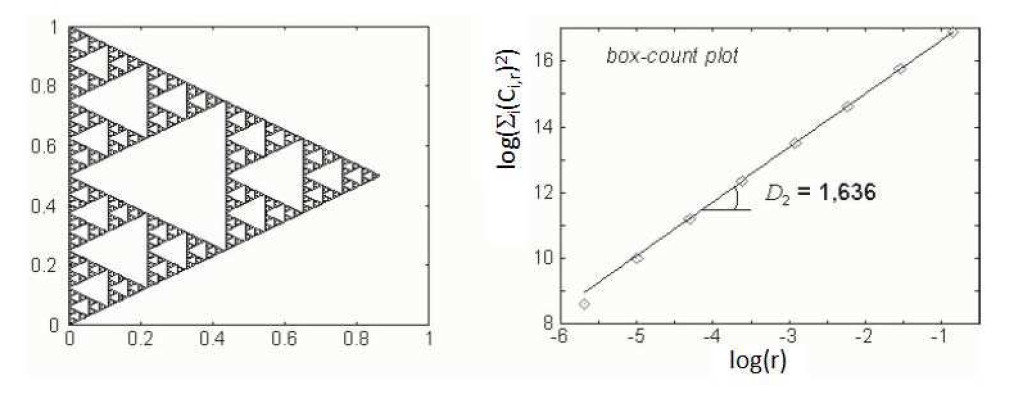
\includegraphics[scale=1.2]{chapter4/ima4.png}
\caption{el conteo de cajas gráfico para el triangulo de sierpinki}
\label{fig:ima4}
\end{figure}

La dimensión fractal fue calculada por el algoritmo Liboc () (coste lineal en el
Número de elementos en el conjunto de datos) presentado en (Traina Jr. et al., 2000, 2010) y presentado como sigue. Considere el espacio de direcciones de un conjunto de puntos en un espacio E-dimensional,
E imponer una rejilla-E con celdas de rejilla de tamaño lateral $r$. Centrándose en la i-ésima célula, deje que $ C_{r,1}$ ser
El recuento ( 'ocupaciones') de puntos en cada celda. A continuación, calcule el valor $\sum_i C_{r,1}^2$

\\\\

La dimensión fractal es la derivada de log $(S (r))$ con respecto al logaritmo de la
radio. Así, el algoritmo de Liboc puede obtener la dimensión fractal D de un conjunto de datos que traza
$S(r)$ en escalas log-log para diferentes valores del radio $r$, y calculando la pendiente de la
Línea resultante.
\\\\

Es necesario procesar $S(r)$ para una cantidad R de valores de r, por lo que el algoritmo puede lograr
Una aproximación estadística adecuada de la línea. Para evitar leer el dataset de nuevo para cada
Valor del radio, Traina Jr. et al. (2010) propuso crear una estructura de cuadrícula de niveles múltiples,
Donde cada nivel tiene un radio la mitad del tamaño del nivel anterior $(r = 1, 1/2, 1/4, 1/8, Etc). $
\\\\

Cada nivel de la estructura corresponde a un radio diferente, por lo que la profundidad de la
Estructura es igual al número de puntos en el gráfico resultante. La estructura se crea
En la memoria principal, por lo que el número de puntos en el gráfico está limitado por la cantidad de
Memoria disponible. Si este gráfico es lineal para un rango adecuado de radios, el conjunto de datos es un
Fractal y su dimensión fractal D es la pendiente de la línea de ajuste de este gráfico.
\\\\

Para cada lado de celda dado $r$, sólo las celdas que tienen al menos un punto ya procesado
Se mantienen, contando la suma de ocupaciones $ C_{r,1}$, i de esta celda. De esta manera, cada nuevo
Punto está directamente asociado a una célula en cada nivel, sin necesidad de ser comparado con
Los puntos previamente leídos. La figura \ref{fig:ima5} muestra la estructura utilizada en el algoritmo para conjuntos de datos de 2 y 3 dimensiones.

\begin{figure}[h]
\centering
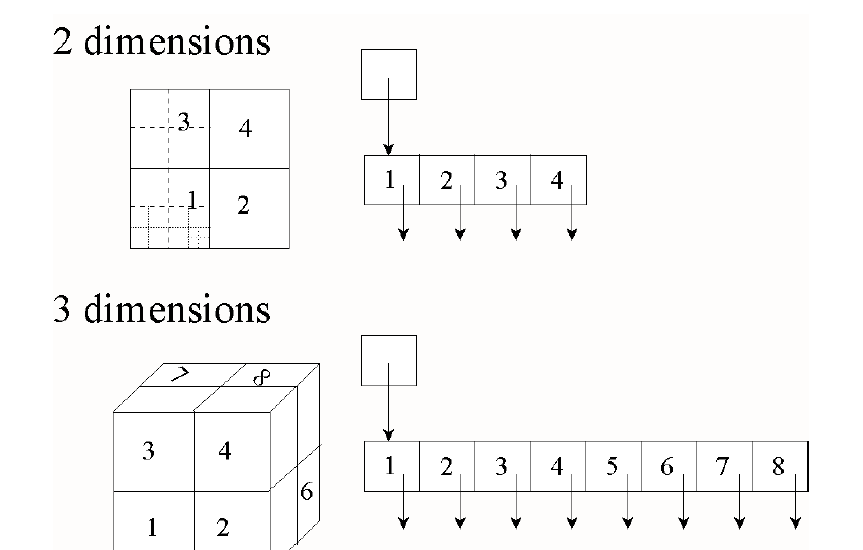
\includegraphics[scale=1.2]{chapter4/ima5.png}
\caption{Representación de las celdas en 2 y 3 dimensiones }
\label{fig:ima5}
\end{figure}
\\\\



El lado de celda más grande del espacio de puntos genera $2^n$ células. En el siguiente nivel, cada
Célula se divide en otras $2^n$ células, y así sucesivamente. Dado que siempre se conoce la posición de cada célula en el espacio, cada célula está representada por: la suma de ocupaciones $ C_{r}$, i en este y los punteros a las celdas en el siguiente nivel cubierto por esta celda (véase la figura 5).
Esta estructura es una especie de $"quad-árbol"$ multidimensional (oct-tree para un espacio 3D, o
E-dim-tree). La figura \ref{fig:ima6}  muestra un ejemplo de esta estructura para un conjunto de datos con cinco puntos
En tres niveles en un espacio bidimensional.
\\\\

\begin{figure}[h]
\centering
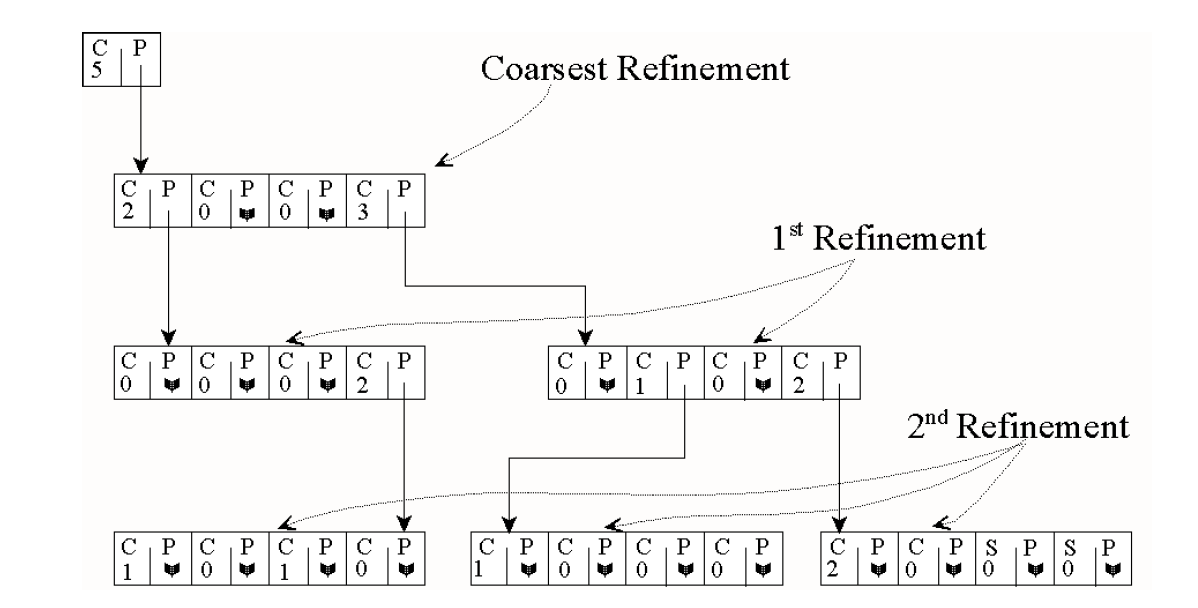
\includegraphics[scale=1.2]{chapter4/ima6.png}
\caption{Ejemplo de los datos estructurados usados para calcular la sumatoria}
\label{fig:ima6}
\end{figure}

\\\\
Observe que se agregan nuevas celdas a la estructura bajo demanda. Así, sólo las células ocupadas
Por al menos un punto $(C_{r,i}> 0)$. El algoritmo procesa sólo los puntos establecidos
Una vez, por lo que es realmente muy rápido. El algoritmo \ref{alg:algo1} resume este proceso de cálculo.
\\\\
\begin{algorithm}
\begin{algorithmic}[1]
\REQUIRE Normalizar el Dataset A(N filas, con E dimensiones/cada atributo)
\label{lin:lineaRara}
\ENSURE  Dimension fractal D
\FOR{Cada tamaño de grid deseaada $r = 1/2^j , j = 1,2, ...,l$}

    \FOR{Cada punto en el dataset}
    \STATE Decide cual celda del grid cae en (la i-esima celda)
    \STATE Incrementa la cuenta $C_i$
    \ENDFOR
    \STATE Procesa la sumatoria de los ocupados $S(r) = \sum C_i^2$
\ENDFOR

\STATE Imprime los valores de $log(r)$ y $log(S(r))$ generando un gráfico

\STATE Retorna la parte linear del gráfico cuesta abajo(regresión linear) de las dimensiones fractales D del dataset A

\end{algorithmic}
\caption{Procesar la dimensión fractal D del dataset A(conteo de cajas aproximadas)}
\label{alg:algo1}
\end{algorithm}

\\\\

En la literatura, existen varios métodos para el cálculo de la dimensión fractal
(Schroeder, 1991, Faloutsos y Kamel, 1994). Sin embargo, el método más adecuado para
El trabajo es el método de recuento de cajas, ya que sólo hemos utilizado conjuntos de datos reales. La correlación dimensión fractal $D_2$ destaca por su relevancia práctica y teórica. Experimentalmente, el cálculo de $D_2$ para fractales estadísticamente auto-similares es relativamente simple, y adecuarlos principalmente para los fractales formados por puntos aislados distribuidos en algunas regiones del espacio donde están inmersos. En teoría, $D_2$ está relacionada con el concepto de correlación,como se describe en la siguiente sección.

\section{Detección de correlación: algoritmo FD-ASE}

El número de atributos en un conjunto de datos determina su dimensión $E$ incrustada, pero si
Hay atributos correlacionados, su dimensión intrínseca $D$ es menor que $E (D < E)$
(Faloutsos y Kamel, 1994). La dimensión intrínseca estimada por el Correlación Fractal
L
\\\\
La función de a dimensión $D_2$ indica el número mínimo de atributos necesarios para representar un conjunto de datos.techo de la dimensión intrínseca $([D])$ determina un umbral superior para
La cantidad de atributos necesarios para representar las características fundamentales del conjunto de datos.
\\\\
$D$ también se puede usar para descubrir cuántos y qué atributos pueden ser empleados para
Reducir la dimensionalidad de los datos. Con este propósito, Sousa et al. (2007b) propuso la FDASE
(Estimador de significación de atributo de dimensión fractal), con el objetivo de identificar
Diferentes tipos de correlaciones. Esta técnica aplica la inclusión de atributo directo
Enfoque y utiliza la dimensión intrínseca como criterio para identificar grupos de
Y seleccionar un subgrupo de atributo relevante para representar los datos esenciales
Características. Las siguientes definiciones son necesarias para comprender mejor la técnica
\\\\

\textbf{Definición 3.5 Dimensión intrínseca parcial $pD():$} Dado un conjunto finito de datos $A = {A_1, a_2,. . . , A_E}$ con atributos E y un subconjunto de atributos $C \subset A$, el intrínseco parcial
La dimensión $pD (C)$ es la dimensión intrínseca que proyecta el conjunto de datos en el subconjunto $C$.


\textbf{Definición 3.6 Contribución individual $iC()$: }Dado un conjunto finito de datos $A = {A_1, a_2,. . . , A_E}$ con atributos $E$, la Contribución Individual $iC()$ de un atributo $a_k \in A $
Es la contribución potencial máxima de $a_k$ a la dimensión intrínseca de $A$, y es
Medida como $ i_C(a_K) = p_D({a_K})\rightarrow [0,1]$.

\\\\
Consideremos un conjunto de datos A y un subconjunto de atributos  $C \subset A$con dimensión intrínseca parcial
$pD (C)$. Un atributo $a_i \in (A - C)$ aumenta la dimensión intrínseca parcial de $ C$ por la mayor parte de su contribución individual $i_C (a_i)$, según el nivel de correlación entre $a_i$ y los atributos de $C$. Si $a_i$ está completamente no correlacionado con cada atributo en $C$,
La dimensión intrínseca parcial aumentará por la contribución individual  $i_C (a_i)$, es decir, $p_D(C \cup{a_i} - p_D(C)\cong iC (a_i)$ Por otro lado, si $ai$ está fuertemente correlacionado con el atributos en $C$, la dimensión intrínseca parcial aumentará en un valor de casi cero, es decir, $p_D(C \cup{a_i} - p_D(C)\cong 0$. Además, si $ai$ está débilmente correlacionado con los atributos en $C$, la dimensión intrínseca parcial aumentará en una cantidad entre cero y la contribución individual $iC (a_i)$, es decir,$0\leq pD(C\cup{a_i}) -pD(C) \leq iC(a_i)$.

\\\\
Correlaciones significa que el valor de un atributo puede ser aproximado de otros
Atributos Sousa et al. (2007b) definieron los términos "correlación fuerte" y "correlación débil".
\\\\
El primero se utiliza cuando el valor de un atributo puede deducirse un subconjunto de otros atributos, como en las correlaciones lineales. Una correlación débil indica que
Un atributo sólo puede ser aproximado de otros atributos, como en las correlaciones fractal.
\\\\

Con el fin de cuantificar la correlación entre los atributos, un umbral $\xi$ varía de cero - que significa correlación completa - hasta uno, cuando los atributos son totalmente independientes.


\textbf{Definición 3.7 $\xi$-Correlación:} Dado un conjunto de datos definido en $A = {A_1, a_2,. . . , A_E}$, a
Se dice que el subconjunto $B\subset A$ está correlacionado con $\xi$ con un subconjunto$C\subset A,B\cap A= \oslash$i cada atributo $a_i$
En $B$ no contribuye más que  $ \xi- ∗ i_C(a_i)$  a la dimensión intrínseca parcial de $C$.

\textbf{Definición 3.8 Conjunto de atributos Núcleo $\xi C$:} Dado un conjunto de datos definido en $A = {A_1, a_2,. . . , A_E}$ con dimensión intrínseca $D$, un Conjunto de Atributos Core $\xi C$es un subconjunto de atributos en $ A$ tales que$\mid pD (\xi C) -D\mid <\exists M_k,M_k(\xi B_P)\rightarrow a_k$, y no hay atributo $ a_k \in \xi C$ tal que $ $.


\textbf{Definición 3.9 Base de correlación $\xi B_p$: }Dado un conjunto de datos  definido en $A = {A_1, a_2,. . . , A_E}$
Y un núcleo de conjunto de atributos $ \xi B_p \subseteq A $, una base de correlación $ xi B_p $ es un subconjunto de atributos $\exists B_p \in (A- \xi C)\mid \exists M_k, M_k(\xi B_p)\rightarrow a_k$ o no hay $\xi$-
Correlacionados en el conjunto de datos y $\xi B_p = \xi C = A$, donde $M_k$ es una correlación que indica
Que ak está $\xi$-correlacionado con todos los atributos en $\xi B_p$.


\textbf{Definición 3.10 Grupo de correlación $\xi  G_p$:} Dado un conjunto de datos definido en $A = {A_1, a_2,. . . , A_E}$ y una Base de Correlación ξBp ⊆ A, un Grupo de Correlación $\xi  G_p$ es el subconjunto
De los atributos $\textbf{ξGp ⊆ A}$, tales que, ξGp = ξBp∪ ak ∈ (A-ξC) | | PD (ξGp) -pD (ξGp-ak) | <
Ξ * iC ({ak}) y ∃Mk (ξBp) → ak, donde Mk es una correlación que indica que ak es ξ-correlacionada
A todos los atributos en ξBp.




